\documentclass[12pt,a4paper,openright,twoside]{book}
\usepackage[utf8]{inputenc}
\usepackage{disi-thesis}
\usepackage{code-lstlistings}
\usepackage{notes}
\usepackage{shortcuts}
\usepackage{acronym}
\usepackage{comment}

\school{\unibo}
\programme{Corso di Laurea Magistrale in Ingegneria e Scienze Informatiche}
\title{Fancy Title}
\author{Penazzi Paolo}
\date{\today}
\subject{Supervisor's course name}
\supervisor{Prof. Supervisor Here}
\cosupervisor{Prof. CoSupervisor 1}
\session{III}
\academicyear{2022-2023}

% Definition of acronyms
\acrodef{CAS}{Collective Adaptive System}
\acrodef{vm}[VM]{Virtual Machine}


\mainlinespacing{1.241} % line spacing in main matter, comment to default (1)

\begin{document}

\frontmatter\frontispiece

\begin{abstract}	
Max 2000 characters, strict.
\end{abstract}

%----------------------------------------------------------------------------------------
\tableofcontents   
\listoffigures     % (optional) comment if empty
\lstlistoflistings % (optional) comment if empty
%----------------------------------------------------------------------------------------

\mainmatter

%----------------------------------------------------------------------------------------
\chapter{Introduction}
\label{chap:introduction}
%----------------------------------------------------------------------------------------

\begin{comment} 
Write your intro here.
\sidenote{Add sidenotes in this way. They are named after the author of the thesis}

You can use acronyms that you defined previously,
such as \ac{IoT}.
%
If you use acronyms twice,
they will be written in full only once
(indeed, you can mention the \ac{IoT} now without it being fully explained).
%
In some cases, you may need a plural form of the acronym.
%
For instance,
that you are discussing \acp{vm},
you may need both \ac{vm} and \acp{vm}.

\paragraph{Structure of the Thesis}

\note{At the end, describe the structure of the paper}

\end{comment}

%----------------------------------------------------------------------------------------
\chapter{Motivation, Background and Related Work}
%----------------------------------------------------------------------------------------

%----------------------------------------------------------------------------------------
\chapter{Analysis}
%----------------------------------------------------------------------------------------

\section{Ubiquitous Language}

To better understand the problem domain and to avoid misunderstandings, a ubiquitous language was defined.

\begin{table}[]
    \begin{tabular}{|l|l|}
    \hline
    \multicolumn{1}{|c|}{\textbf{Term}} & \multicolumn{1}{c|}{\textbf{Meaning}}                                                                                                                                                               \\ \hline
    Testing                             & The overall process carried out to verify and validate a system, according to requirements, to promote the desired internal and external quality and to mitigate risks in development and products. \\ \hline
    Testbed                             & A platform for rigorous transparent and replicable environment for experimentation and testing TODO Cite                                                                                            \\ \hline
    Solution                            & Consist of a set of algorithms leading to achieving goals and overcoming the problem posted                                                                                                         \\ \hline
    Scenario                            & Contains all the information about the test execution: the simulation platform, the metrics, the input parameters                                                                                             \\ \hline
    Simulator                           & A software that allows the user to see how its program would behave in a real environment                                                                                                                     \\ \hline
    Parser                              & Component of the Testbed responsible for the read of the input file                                                                                                                                           \\ \hline
    Listener                            & Component of the Testbed responsible for the read of the output of the simulator                                                                                                                              \\ \hline
    \end{tabular}
    \end{table}

\section{Technologies}

\subsection{Containerization}
% What is containerization
Containerization is a lightweight alternative to full-machine virtualization that involves encapsulating 
an application in a container with its own operating environment.
% Why containerization is needed
The main reason for using containerization is to create a consistent, isolated environment for applications to run in.
By doing so, the user can be sure that the application will always run the same way, regardless of the user's machine configuration. 
Further, this allows the user to focus solely on the application itself, without having to worry about dependencies, software updates, compatibility and things like this.
% Choice of Docker as containerization technology
When choosing a containerization technology, the choice was between the two most popular solutions in this field: Docker and Kubernetes.
Ultimately, Docker was chosen because it is more lightweight and easier to use than Kubernetes.
% How Docker works
Docker is a platform for building, running, and shipping applications in containers.
Docker containers wrap up a piece of software in a complete filesystem that contains everything it needs to run:
code, runtime, system tools, system libraries - anything you can install on a server.
To create a container, a Dockerfile is needed, which is a text document that contains all the 


\subsection{Language}
Different languages were considered for the implementation of the system.

\paragraph*{Scala}
Scala is a strong statically typed high-level general-purpose programming language that supports both object-oriented 
programming and functional programming. 
Designed to be concise, scalable and safe, many of Scala's design decisions are aimed at addressing criticisms of Java.
\cite{enwiki:1179700699}
One weakness of Scala is its steep learning curve, which makes it difficult to learn for new users.

\paragraph*{Kotlin}
Kotlin is a cross-platform, statically typed, general-purpose high-level programming language with type inference. 
Kotlin is designed to interoperate fully with Java.
Support for multiplatform programming is one of Kotlin’s key benefits. It reduces time spent writing and maintaining 
the same code for different platforms while retaining the flexibility and benefits of native programming.
%[https://github.com/JetBrains/kotlin]

\paragraph*{Rust}
Rust is a multi-paradigm programming language designed for performance and safety, especially safe concurrency.
It has been designed to be a safe, concurrent, practical language, supporting functional and imperative-procedural paradigms.
It is considered the modern version of C and C++.

\paragraph*{Final choice}
After a brief analysis, it was clear that both Kotlin and Scala were suitable candidates for the implementation of the system.
In the end, the choice fell on Scala, because the author had previous experience with it.

%----------------------------------------------------------------------------------------
\chapter{Design}
%----------------------------------------------------------------------------------------

%----------------------------------------------------------------------------------------
\chapter{Implementation}
%----------------------------------------------------------------------------------------

%----------------------------------------------------------------------------------------
\chapter{Evaluation}
%----------------------------------------------------------------------------------------

%----------------------------------------------------------------------------------------
\chapter{Conclusion and Future Work}
%----------------------------------------------------------------------------------------

\begin{comment}

I suggest referencing stuff as follows: \cref{fig:random-image} or \Cref{fig:random-image}

\begin{figure}
    \centering
    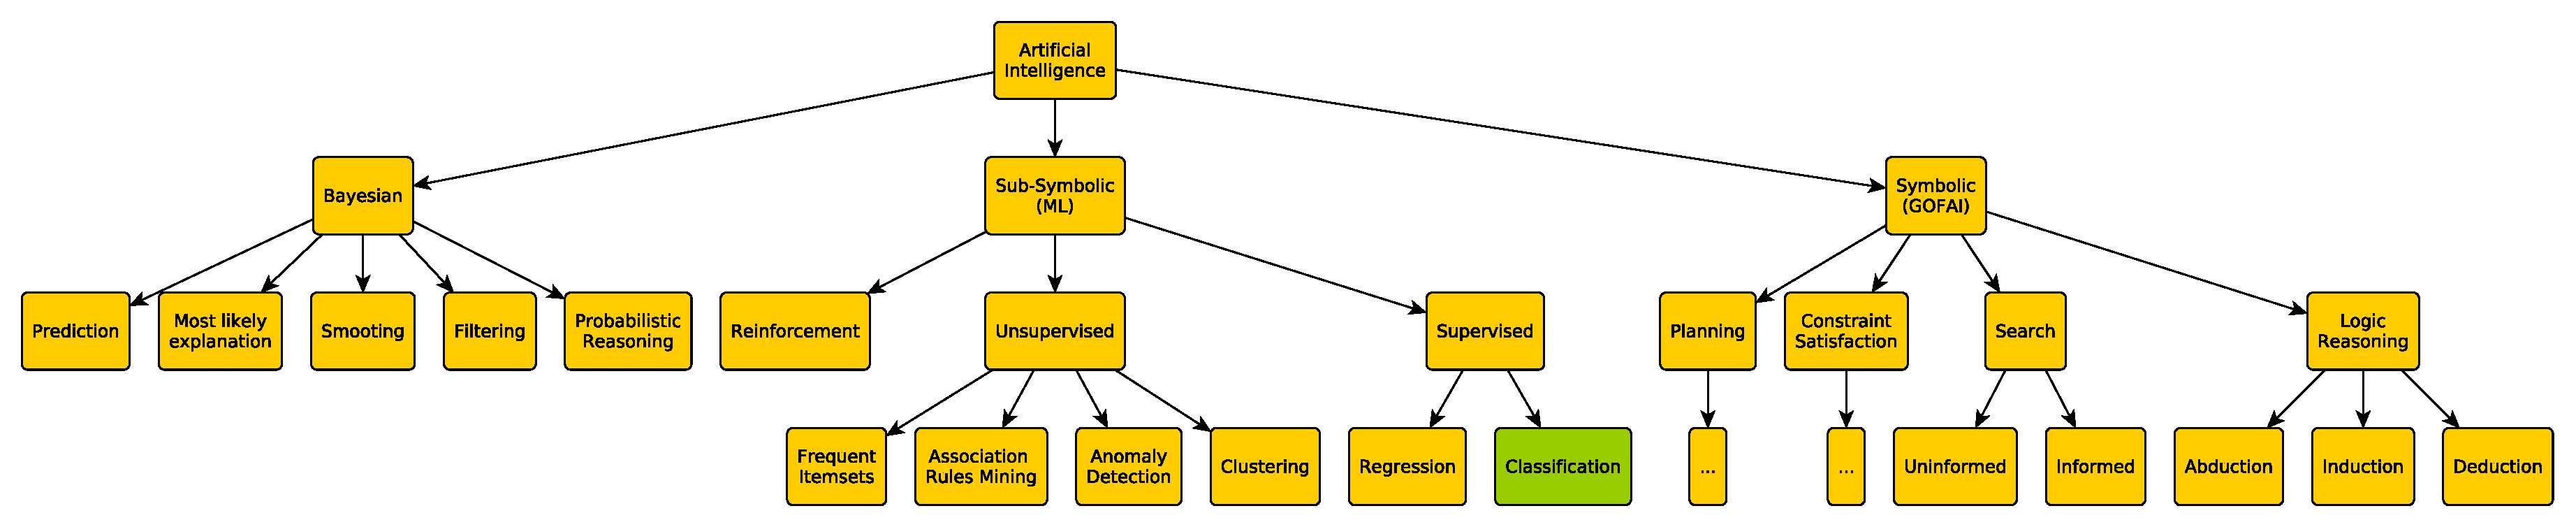
\includegraphics[width=.8\linewidth]{figures/random-image.pdf}
    \caption{Some random image}
    \label{fig:random-image}
\end{figure}

\section{Some cool topic}

You may also put some code snippet (which is NOT float by default), eg: \cref{lst:random-code}.

\lstinputlisting[float,language=Java,label={lst:random-code}]{listings/HelloWorld.java}

\section{Fancy formulas here}

\end{comment}

%----------------------------------------------------------------------------------------
% BIBLIOGRAPHY
%----------------------------------------------------------------------------------------

\backmatter

\nocite{*} % comment this to only show the referenced entries from the .bib file

\bibliographystyle{alpha}
\bibliography{bibliography}

\end{document}